\documentclass[11pt]{report}

\usepackage[toc,page]{appendix}
% CPS equations
\usepackage{amsmath}
\usepackage{stmaryrd}
% Grammar
\usepackage{syntax}
% Operational semantics
\usepackage{semantic}
% Stages diagram
\usepackage{tikz}
% Stages diagram elements
\usepackage{graphicx}
% Chapter number and name on one line
\usepackage{titlesec}
\titleformat{\chapter}[hang] 
{\normalfont\huge\bfseries}{\thechapter}{1em}{} 
% No new page after chapter
%\usepackage{etoolbox}
%\makeatletter
%\patchcmd{\chapter}{\if@openright\cleardoublepage\else\clearpage\fi}{}{}{}
%\makeatother
% Source code listings
\usepackage{listings}
\lstset{frame=single, numbers=left, basicstyle=\ttfamily}
% Line spacing
\usepackage{setspace}
% AST example
\usepackage{qtree}

%%%%%%%%%%%%%%%%%%%%%%%%%%%%%%%%%%%%%%%%%%%%%%%%%%%%%%%%%%%%%%%%%%%%%%%%%%%%%%%%%%%%%%

\title{LJSP - A LISP to asm.js compiler}
\author{Jan S\"ondermann}
\date{1st January 1900}

% Commands to make CPS equations easier to write
\newcommand{\eqdef}{\stackrel{\text{def}}{=}}%
\newcommand{\cpstrans}[1]{\ensuremath{\mathcal{K}\llbracket #1 \rrbracket}}

%%%%%%%%%%%%%%%%%%%%%%%%%%%%%%%%%%%%%%%%%%%%%%%%%%%%%%%%%%%%%%%%%%%%%%%%%%%%%%%%%%%%%%

\begin{document}
% TODO why scala? why LLVM IR/C
% TODO mention that LJSP is a subset of Scheme
% TODO consistent spelling of "JavaScript"


\maketitle

\onehalfspacing

\begin{center}
\textbf{Originality avowal}
\end{center}

I verify that I am the sole author of this report, except where explicitly stated to the contrary.

I grant the right to King's College London to make paper and electronic copies of the submitted work for purposes of marking, plagiarism detection and archival, and to upload a copy of the work to Turnitin or another trusted plagiarism detection service.

\begin{flushright}
Jan Söndermann \\
@@date@@@
\end{flushright}
\newpage
			
\begin{center}
\textbf{Abstract}
\end{center}

@@@
\newpage

\begin{center}
\textbf{Acknowledgements}
\end{center}
I would like to thank my supervisor Dr. Christian Urban for supervising my project and for providing me with both guidance and freedom.
\newpage

\tableofcontents
\newpage

\chapter{Introduction}
One of the main trends of today's Internet is the shift from traditionally offline or standalone programs to the web. This phenomenon, often called "Web 2.0" is exemplified in the success of web applications such as GMail and Facebook.

This success of the web has brought with it the rise of the programming language it is build on: JavaScript, the only language that is supported by all major browsers. Statistics, such as the number of repositories created on GitHub (a popular code sharing website) using JavaScript, reflect this success: in 2013, JavaScript led this list by a substantial margin \cite{githubarchive} \cite{topgithub}.

% TODO possibly add refs to ember, meteor websites
Since JavaScript is no longer confined to being used for simple animations and input-validation tasks, the complexity of web apps has increased tremendously. Modern JavaScript frameworks, such as Ember.js link or Meteor use the full register of functionality the language offers and are just as complex as traditional web frameworks that use other languages such as Ruby or Python.

% TODO possibly provide citation for the consensus claim
Unfortunately, this proliferation of JavaScript has taken the language far beyond the tasks it was initially conceived for. There is a widespread consensus that the language has a number of shortcomings. Brendan Eich, the creator of JavaScript, writes\cite{brendeich} about its early history:
\begin{quote}
In April 1995 I joined Netscape in order to "add Scheme to the browser." [...]

So in 10 days in May 1995, I prototyped "Mocha," the code name Marc Andreessen had chosen. [...]

To overcome all doubts, I needed a demo in 10 days. I worked day and night, and consequently made a few language-design mistakes (some recapitulating bad design paths in the evolution of LISP), but I met the deadline and did the demo.
\end{quote}

Criticism of JavaScript has mostly focussed on two areas:
\begin{itemize}
\item Inconsistencies and mistakes in the design of the language. Examples given for this often include the confusion around JavaScript's large number of falsy values (\texttt{0},  \texttt{''}, \texttt{NaN}, \texttt{false}, \texttt{null} and \texttt{undefined}) and its set of reserved keywords, which includes a large number of words not in use by the language but doesn't include \texttt{NaN} and \texttt{undefined}. This makes it necessary to test for \texttt{undefined}ness using \\
\mbox{\texttt{typeof x === 'undefined'}} to avoid comparing against a redefined \texttt{undefined}. For more examples, see the excellent \cite{jsgoodparts}.
% TODO give citation/explanation for the dynamic claim
\item Slow execution speed. Writing fast interpreters for JavaScript has been an extraordinary difficult task for browser manufacturers. This is due to the extremely dynamic nature of JavaScript.
\end{itemize}

% TODO don't cite jsgoodparts twice (below and above)
% TODO possible add links to coffeescript etc.
Programmers have responded to the first problem in ways that include limiting themselves to a subset of JavaScript that excludes the inconsistent and badly-designed parts (cf. the very popular "JavaScript: The Good Parts" \cite{jsgoodparts}). Another response has been to create new languages that compile to JavaScript, such as the very popular CoffeeScript, Microsoft's TypeScript and Google's Dart.

The second problem has been partly remedied by a new generation of JavaScript engines spearheaded by Google's V8, released in 2008 as part of Google Chrome. The other browser makers, including Mozilla soon followed by rewriting their own JavaScript engines. These new engines often brought impressive speed gains.

In early 2013, Mozilla released asm.js, a project that claims to take these two approaches to their logical conclusion. It defines an extremely limited, statically typed subset of JavaScript that can be executed very quickly. This subset is intended as compilation targets for high level languages.

The goal of this project is twofold
\begin{itemize}
\item To design such a high level and provide a compiler for it that compiles the language to asm.js.
\item To test the performance of this new language that we called LJSP and compare it to plain JavaScript.
\end{itemize}

To achieve the second goal, the project includes a ray tracer in JavaScript, parts of which were rewritten in LJSP and compiled to asm.js. Rendering time of a 3D scene functioned as a benchmark that made it possible to evaluate the results of the project.

% TODO history. also include ray tracer

\chapter{Background}
This chapter will describe the background and context of the LJSP project. It will give an appropriate level of technical details of the technologies involved in the compiler and justify the motivation for starting this project.

\section{asm.js}
% TODO add reference to asm.js spec

Asm.js is a small subset of JavaScript that can be compiled to very fast machine code. Benchmarks show \cite{asmjsbenchmark} running times around twice the speed of native code. To showcase the speed of asm.js, researches at Mozilla compiled the Unreal gaming engine to asm.js, producing smooth and stutter free rendering inside the browser \cite{unreal}.

The development and release of asm.js is the main motivation of the LJSP project. The goal of LJSP is to evaluate the performance achievable with a language that compiles to asm.js. This section will describe the concepts behind asm.js and give a technical description of its specification. The Implementation chapter below will build on this description to explain the asm.js code that the LJSP compiler outputs.

Asm.js is designed as a very limited subset of JavaScript that includes information typically not included in JavaScript code. If the author of a function written as asm.js compatible code adds a statement that makes the function as compatible, and the browser of the user viewing a website that includes this code supports asm.js, the JavaScript engine of the browser can use that additional information to compile the code to very efficient Assembly.

The way to opt-in to this optimisation is to add a \texttt{"use asm";} statement to the top of the function\footnote{The syntax for this opt-in is copied from the popular and widespread \texttt{"use strict";} that makes JavaScript engines less lenient when parsing JavaScript code.}. Supporting browsers (currently only Firefox) will then compile the code and output a notice such as "\texttt{successfully compiled asm.js code (total compilation time 25ms)}" in the case of successful compilation to the console when encountering this function.

Most of the additional information that asm.js forces the programmer to include in his programs that would typically not be part of idiomatic JavaScript is type information. Unlike JavaScript, asm.js is statically typed, meaning every variable has a type inferable at compile time. The following examples will illustrate this difference. We start with a small function in standard Javascript).

% TODO enclose all listings in figures
\begin{lstlisting}
function add(a, b) {
    return a + b;
}
\end{lstlisting}

The name of this function suggests that it was probably conceived to add two numbers. It could, however, be called with \texttt{add("hello ", "world");} and would yield the string \texttt{"hello world"}. Neither is it restricted in the type of numbers it accepts: it can be called with an arbitrary combination of integers and floating point numbers.

The same function restricted to integers in asm.js would look as follows:

\begin{lstlisting}
function add_ints(a, b) {
    a = a|0;
    b = b|0;
    
    return (a + b)|0;
}
\end{lstlisting}

The additional lines 2 and 3 are the abovementioned type information. They declare both parameters \texttt{a} and \texttt{b} to be of type int. In other languages such as C, this would be written as \texttt{int a, int b}. In valid asm.js, all parameters to every function get a type assigned in this way.

The other change from the original JavaScript version to the asm.js version of the add function is the addition of a bitwise or with 0 to the result of the addition in line 5. This is necessary because of the other main feature of asm.js besides the possibility of compiling it efficiently. 

% TODO add link to the js spec
The asm.js specification guarantees that valid asm.js code evaluates to the same result regardless of whether or not the browser has asm.js support. If we consider the situation where the browser does have asm.js support and the function \texttt{add_ints} defined in the example above is called with two very large integers, the compiled, native code would add these two large ints and cause an integer overflow. If, however, the browser does not support asm.js and treats the code as normal JavaScript, adding two integers large enough that normally an overflow would occur causes the result to be cast to a floating point number according to the JavaScript specification.

% TODO "not defined" is probably not correct. better: make no sense
The bitwise or in the line \texttt{return (a + b)|0;} ensures that even in the case of missing asm.js support, the result returned by the function would still be an overflowed integer. The reason for this is that the bitwise or with 0 coerces the result to be of type int, because bitwise operations on floating point numbers are not defined. These expressions are therefore known as "type coercions" and asm.js makes heavy use of them.

To illustrate type coercions with an example, consider the following interactive JavaScript session:

\begin{lstlisting}
> 2147483647 + 1
2147483648
> (2147483647 + 1) |0
-2147483648
\end{lstlisting}

$2147483647$ is equal to $2^{31}-1$, the largest value that can be saved in a 32 bit signed integer variable. If we add one to this value without any coercion, the result is transparently cast to a double and returned. If, however, we include a type coercion, the result overflows to $-2^{31}$.

To conclude this section, we will give an overview of the asm.js specification with a restriction on the parts that are relevant to the LJSP compiler. For reasons of length, this overview will leave out information that is unimportant for the project and is not meant as a general introduction to asm.js.

Asm.js code is organised in asm.js modules which consist of a function that includes the \texttt{"use asm";} statement mentioned at the beginning of this section. As parameters, it can take a stdlib object that makes it possible to import certain functions from the JavaScript standard library into the asm.js module and an ArrayBuffer\footnote{In JavaScript, ArrayBuffer objects represent blocks of memory. These blocks can be used with views, such as Int32Array, that declare the content of the memory to be of a specific type.} object often called "heap". Besides this, it can also include:
\begin{itemize}
\item Global variables
\item Functions
\item Function tables
\item A return statement
\end{itemize}

Valid asm.js functions include enough type information to be statically typable as explained above. They can declare variables, perform arithmetic operations on these variables, branch using \texttt{if} statements, read from and write to the heap and call functions either by name or by looking them up in a function table.

Function tables in asm.js are arrays of functions. These arrays must be of a length equal to a power of two. When using a function table to call a function, the variable that is used as index must be masked bitwise to ensure that function table lookup never failes with an out of bounds error. This is a complex idea best illustrated with an example. Assume our code includes a function table \texttt{ftable} that contains $8$ functions, and a variable \texttt{x} that holds the index to a function in \texttt{ftable} that we would like to call. This call could be achieved with the statement \texttt{ftable[x \& 7](param1, param2, ...);}. The bitwise AND with $7$ (equal to \texttt{ftable.length - 1}) ensures that regardless of the value \texttt{x} holds, no out of bounds error can occur. The reason asm.js allows multiple function tables is because all functions in a table must have the exact same type signature in parameters and return types.

The return statement at the end can make functions defined inside the module visible to the outside.

\section{LLVM and Emscripten}
% TODO cite LLVM paper
% TODO mention some of the more obscure uses of LLVM
% TODO give examples of LLVM IR code
LLVM is a compiler project that includes and has spawned a large number of tools and programs related to the compilation of programs. At its core, it defines an intermediate representation called LLVM IR and an optimizer for this language. This intermediate representation aims to be a shared interface for front ends that parse programming languages and compile them to LLVM IR and back ends that take LLVM IR code and produce native code for a specific architecture such as x86 or arm. 

% TODO cite paper on emcc (on desktop)
While a large number of these front and back ends for various languages and architectures have been written, only one is relevant to the LJSP project: a LLVM IR to JavaScript compiler called Emscripten. Emscripten was written by the same people that invented asm.js, in fact, asm.js was created to fill a need the Emscripten developers had for a better compilation target.

The LJSP compiler emits both C and LLVM IR code. This generated code can be compiled with Emscripten to asm.js. The Evaluation chapter will compare the running time of this code that Emscripten emits with the asm.js code that LJSP generates directly.

\section{Ray tracing}
Ever since the first computer were built, programmers have sought ways to generate pictures with programs. Especially with the rise of computer games, this has become a heavily researched area. Ray tracing is one such technique to generate images from description of 3D scenes.

Before we describe the details of ray tracing, we have introduce two terms that we will refer to in our explanation: A \textbf{3D Scene} is an arrangement of objects at specific coordinates in 3D space. Object can include shapes such as spheres, cubes or planes, lights and a camera. The \textbf{camera} is not a visible object, but instead gives the perspective an angle from which the scene will be rendered. This is also commonly referred to as "eye". \textbf{Rendering} denotes the process of generating an image from a 3D scene and the program that does this is called a renderer.

Ray tracing produces relatively impressive results with simple techniques. It works by shooting rays from the eye into the scene. The ray tracer then traces these rays and determines whether they hit an object in the scene. If they do, the process of shooting rays into the scene is repeated recursively with the intersection point as the origin of the rays to achieve photorealistic effects such as reflection. If they don't, black or some other background colour is displayed.

This idea is illustrated by figure \ref{raytracingexplanation}.

% TODO make a diagram that explains ray tracing
\begin{figure}[ht]
%\includegraphics{asdf.eps}
\caption{Tracing rays}
\label{raytracingexplanation}
\end{figure}

% TODO possibly include this at the end if not at word limit yet
%    \section{Similar Languages}
% lisps that compile to js but also coffeescript, dart, etc.


\chapter{Requirements}

\chapter{Specification}
\section{Grammars}
\subsection{LJSP Grammar}
The grammar of LJSP in Extended Backus-Naur Form is given below.

\begin{grammar}
<program> ::= <defines> [ <expr> ] <defines>

<defines> ::= <define> <defines> | $\epsilon$

<define> ::= `(define (' <ident> <params> `)' <expr> `)'

<expr> ::= <double>
\alt <ident>
\alt `(if' <expr> <expr> <expr> `)'
\alt <lambda>
\alt `(let (' <letblocks> `)' <expr> `)'
\alt `(' <primOp> <args> `)'
\alt `(' <expr> <args> `)'

% add scientific form
<double> ::= \texttt{-?(\textbackslash d+(\textbackslash.\textbackslash d*)?|\textbackslash d*\textbackslash.\textbackslash d+)}

<ident> ::= \texttt{[a-zA-Z=*+/\textless\textgreater!?-][a-zA-Z0-9=*+/\textless\textgreater!?-_]*}

<lambda> ::= `(lambda (' <params> `)' <expr> `)'

<params> ::= <ident> | <ident> <params>

<letblocks> ::= <letblock> | <letblock> <letblocks>

<letblock> ::= `(' <ident> <expr> `)'

<primOp> ::= `+' | `-' | `*' | `/' | `neg'
\alt `>=' | `<=' | `=' | `not' | `<' | `>' | `and' | `or'
\alt `min' | `max'
\alt `sqrt'

% is an application to an empty argument list legal?
<args> ::= <expr> | <expr> <args>
\end{grammar}

The grammar for LJSP expressions used in the front end stages is as follows:
\begin{grammar}
<expr> ::= <env>
\alt `(make-closure' <lambda> <env> `)'
\alt `(nth' <int> <expr> `)'
\alt `(get-env' <expr> `)'
\alt `(get-proc' <expr> `)'
% should this be <expr> instead of <env>?
\alt `(hoisted-lambda' <ident> <env> `)'

<env> ::= `(make-env' <idents> `)'

<int> ::= \texttt{-?(0|[1-9][0-9]*)}

<idents> ::= <ident> <idents> | $\epsilon$
\end{grammar}

\subsection{Grammar of the Intermediate Representation (IR)}
The grammer for the Intermediate Representation of the LJSP compiler is given below.
\begin{grammar}
<iModule> ::= <iFunctions>

<iFunctions> ::= <iFunction> <iFunctions> | $\epsilon$

<iFunction> ::= `function' <ident> `(' <params> `)' `{' <iStatements> `}'

<iStatements> ::= <iStatement> <iStatement> | $\epsilon$

<iStatement> ::= <ident> `=' <iExpr>
\alt `if (' <ident> `) {' <iStatements> `} else {' <iStatements> `}'
\alt <iExpr>

<iExpr> ::= <ident>
\alt <double>
\alt <ident> `(' <iArgs> `)'
\alt <iUnaryPrimOp> <iExpr>
\alt <iExpr> <iBinaryPrimOp> <iExpr>
\alt `make-env(' <iIdents> `)'
\alt `make-hl(' <ident> `,' <ident> `)'
\alt <ident> `[' <index> `]'

<iArgs> ::= <iExpr> | <iExpr> <iArgs>

<iUnaryPrimOp> ::= `sqrt'

<iBinaryPrimOp> ::= `+' | `-' | `*' | `/'
\alt | `==' | `<' | `>'
\alt `min' | `max'

<iIdents> ::= <ident> | <ident> <iIdents>

<index> ::= \texttt{0 | [1-9][0-9]*}


\end{grammar}


% IR grammar

% grammar of intermediate representation, C?

% subset of scheme
\section{Small-Step Semantics of LJSP}
In this section, we give the small-step semantics of the LJSP language. In the expressions below, $i$ stands for an identifier, $v$ stands for a generic value, $e$ stands for an expression, $c$ stands for a context that an expression is evaluated within and $\Lambda$ stands for a \texttt{(lambda...)} expression.
% TODO maybe change names from func_appl1 to "func appl 1"
\begin{gather*}
\inference[var]{}{\langle i, c \rangle~\rightarrow~\langle v, c\rangle~\text{if}~c(i) = v}\\\\
%
\inference[let1]{\langle e_1, c \rangle~\rightarrow~\langle e_1', c' \rangle}{\langle (\text{let}~i_1=e_1,~\dots~\text{in}~e), c \rangle~\rightarrow~\langle (\text{let}~i_1=e_1',~\dots~\text{in}~e), c' \rangle}\\
%
\inference[let2]{}{\langle (\text{let}~i_1=v,~\dots~\text{in}~e), c \rangle~\rightarrow~\langle (\text{let}~i_2=e_2,~\dots~\text{in}~e, c[i_1 \mapsto v] \rangle}\\
%
\inference[let3]{}{\langle (\text{let}~i=v~\text{in}~e), c \rangle~\rightarrow~\langle e, c[i \mapsto v] \rangle}\\\\
%
\inference[func_appl1]{\langle e, c \rangle~\rightarrow~\langle e', c' \rangle}{\langle (f_{name}~\dots,~e,~\dots), c \rangle~\rightarrow~\langle (f_{name} ~\dots,~e',~\dots), c' \rangle}\\
%
\inference[func_appl2]{}{\langle (f_{name} ~v_1,~\dots,~v_n), c \rangle~\rightarrow~\langle f_{body}, c[f_{param_1} \mapsto v_1,~\dots,~f_{param_n} \mapsto v_n] \rangle}\\\\
%
\inference[lambda_appl1]{\langle l, c \rangle~\rightarrow~\langle \Lambda, c' \rangle}{\langle (l~\dots,~e,~\dots), c \rangle~\rightarrow~\langle (\Lambda~\dots,~e,~\dots), c' \rangle}\\
%
\inference[lambda_appl2]{\langle e, c \rangle~\rightarrow~\langle e', c' \rangle}{\langle (\Lambda~\dots,~e,~\dots), c \rangle~\rightarrow~\langle (\Lambda ~\dots,~e',~\dots), c' \rangle}\\
%
\inference[lambda_appl3]{}{\langle (\Lambda ~v_1,~\dots,~v_n), c \rangle~\rightarrow~\langle \Lambda_{body}, c[\Lambda_{param_1} \mapsto v_1,~\dots,~\Lambda_{param_n} \mapsto v_n] \rangle}\\\\
%
\inference[prim_op1]{\langle e, c \rangle~\rightarrow~\langle e', c' \rangle}{\langle (prim~\dots,~e,~\dots), c \rangle~\rightarrow~\langle (prim~\dots,~e',~\dots), c' \rangle}\\
%
\inference[prim_op2]{}{\langle (prim~d_1,~\dots,~d_n), c \rangle~\rightarrow~\langle d, c \rangle~\text{if}~prim(d_1,~\dots,~d_n) = d}\\\\
%
\inference[if]{\langle e_1, c \rangle~\rightarrow~\langle e_1', c' \rangle}{\langle (\text{if}\ e_1, e_2, e_3), c \rangle~\rightarrow~\langle (\text{if}\ e_1', e_2, e_3), c' \rangle}\\
%
\inference[if(true)]{}{\langle (\text{if}\ \text{\#t}, e_2, e_3), c \rangle~\rightarrow~\langle e_2, c \rangle}\\
%
\inference[if(false)]{}{\langle (\text{if}\ \text{\#f}, e_2, e_3), c \rangle~\rightarrow ~\langle e_3, c \rangle}
\end{gather*}

% TODO Big step semantics

\chapter{Design}
% TODO use transformation, stage, conversion, phase more consistently.
%      conversion: one AST class hierarchy -> another
%      phase: front end/interm./back end

This chapter will describe the design of the LJSP compiler. It will give an abstract, theoretical description of all the subsystems that make up the compiler. The next chapter will then describe the concrete implementation of these subsystems. Together, these two chapters will give the reader a full understanding of the inner workings of the LJSP compiler.

\section{Architecture of the Compiler}
The compiler is made up of two major components: A hierarchy of classes that get instantiated to create an internal representation of the program called the Abstract Syntax Tree (AST) and a large number of compilation stages that perform various transformation on this AST to bring it into a form closer to the desired output.

When compiling a program, the compiler will first create the AST of the input program given. It will then run this AST through a number of stages depending on the desired output (e.g. asm.js or C) before finally converting the resulting AST back to a textual representation.

In the following, we will first describe the AST classes before going through all the individual stages of the compiler in detail.

\subsection{The Abstract Syntax Tree}
% TODO cite: something about ASTs maybe from the dragon book
The Abstract Syntax Tree (AST) is the representation of the program that the compiler uses internally. It gets generated by the first stage, parsing, whose purpose it is to convert the users' textual representation of the program to an AST. Correspondingly, the compiler includes functions that convert an AST back to program code in text form. The details of these conversion will be described in more detail in the implementation chapter.

As its name suggests, the Abstract Syntax Tree is a Tree representation of the code. As an illustration of the structure of these trees, we give the AST for the expression \hbox{\texttt{(* (+ x 1) 2)}} below.

% TODO make a nicer tree with asymptote
\begin{figure}[ht]
\hskip-0.3in
\Tree [.* [.+ x 1 ] 2 ]
\caption{Example of an Abstract Syntax Tree}
\label{astexample}
\end{figure}

% TODO maybe add more complex example and explain in the paragraph below which rule corresponds to which nodes

All nodes in the Abstract Syntax Tree are objects. These objects are instances of classes that very closely reflect the grammar of the language the program that the AST represents is written in. This means that every language used in the LJSP compiler (LJSP itself, the Intermediate Representation described in the next section and all output languages) have their own hierarchy of AST classes. Some compilation stages manipulate the AST without changing the types of the objects its made up of, whereas some convert the AST from one language to another. 

% TODO add diagrams for AST class hierarchies

\subsection{Compilation stages}
% TODO talk about nanostage compiler
% TODO add citation for the "common" claim
Because compiling a program from one programming language to another is often a very complex transformation, it is common to break up this transformations into a number of stages that each accomplish a small part of this overall transformation. While these stages can vary quite significantly in complexity ranging from simple expansions of specific expressions (an example would be converting expressions of the form \hbox{\texttt{1 + 2 + 3 + 4}} to \hbox{\texttt{((1 + 2) + 3) + 4}}) to more complex transformations such as CPS-Translation, they are all of managable complexity when compared to the overall goal of transforming from the input to the output language.

All stages in the compiler take an produce an Abstract Syntax Tree which they manipulate \footnote{An exception to this are the very first and very last stages, whose purpose it is to convert between textual representations of the program and the AST.}. An important observation on compilation stages is that they should not change what the AST evaluates to, i.e. not change the meaning of the program.

Like many other compilers, the LJSP compiler is made up of compilation stages. These stages make up the core of the compiler and will be described in detail the following subsections.

\subsubsection{Overview of compilation stages}

%structure: front end, mid end back end

\begin{figure}[ht]
\begin{center}
\includegraphics[scale=0.8]{stagesflowchart.eps}
\caption{Flowchart for compilation stages in LJSP}
\end{center}
\label{stagesflowchart}
\end{figure}

% TODO the name underneath the figure and the one in the text don't match
% TODO mention special forms that front end stages use and how that's handled in testing
Figure \ref{stagesflowchart} shows all the compilation stages that the LJSP compiler is made up of. These stages  can be grouped into three sections:
\begin{itemize}
\item \textbf{Front end stages}: These first six stages make up the first part of the transformations the code passes through. Their structure is that of a simple list as there is no branching of stages in the front end. These stages all operate on LJSP code, but they all reduce the complexity of the code. Letn expansion and prim op reduction reduce the number of distinct instructions in the code, CPS-translation makes control flow explicit while the latter two stages remove anonymous function objects by turning them into named functions. This reduction of complexity is necessary to bridge the gap between LJSP, a very high-level language that includes such concepts as functions as first class variables, and low-level output languages such as LLVM IR that do not include these concepts. In the diagram, they are depicted as boxes with a green background.

\item \textbf{Intermediate stages}: These stages convert the LJSP AST obtained after passing through the front end stages into a different language called the Intermediate Representation (IR) of the LJSP compiler before performing various optimisations on this IR code. IR is an imperative, untyped language, that is general enough to be converted to both asm.js and C but close enough to these languages to avoid code duplication. This part of the compiler currently consists of two stages, one that converts LJSP to IR and a simple optimisation that removes redundant assignments. It offers a suitable framework for adding additional optimisations that automatically get shared between all output languages. In the diagram, intermediate stages are shown as boxes with a red background.

\item \textbf{Back end stages}: This part of the compiler comprises all the stages that result in an output language. The relationships between these stages are more complex and include some branching, the reasons for which will be described in the section below. In the diagram, back end stages are shown as boxes with a blue background.
\end{itemize}

This subdivision of stages into the three groups described above has been inspired by large, industrial strength compilers such as LLVM.

\begin{figure}[ht]
\begin{center}
% TODO add diagram
\caption{High level overview of LJSP compilation stages}
\end{center}
\label{highlevelstages}
\end{figure}

One important consideration when structuring a compiler in this way is to avoid code duplication. Figure \ref{highlevelstages} shows a high level overview of the compilation stages in the LJSP compiler. It shows that regardless of the possible output languages the user of the compiler chooses, all programs pass through the red, intermediate stages. This makes them ideal for transformations that are shared among all output languages, such as code optimisations. The first implementation of the LJSP compiler did not include any intermediate stages and transformed LJSP ASTs obtained after the front end stages straight to asm.js. After adding additional back ends (C first, later LLVM), however, the need for an Intermediate Representation quickly became obvious due to the large amound of duplicated code.

\section{Detailed description of compilation stages}
We will now describe all the stages of the LJSP compiler in detail. For many stages, this will include a set of equations to define the stages in a precise way. In these equations, $y$ will stands for a variable, $d$ for a double constant and $f$ for a fresh identifier. Functions of the form $\mathcal{A}\llbracket e \rrbracket$ will denote transformation $\mathcal{A}$ applied to expression $e$.

\subsection{Parsing}
This very first stage takes the textual representation of the program and converts it to an Abstract Syntax Tree that the subsequent stages manipulate. It does so according to the grammar of LJSP described in the Specification chapter. Because of its syntax, LJSP is a very easy language to parse, which makes this a relatively simple stage. The details of parsing will be described in the Implementation chapter.

\subsection{\texttt{letn} expansion}
\begin{figure}[ht]
\begin{alignat*}{2}
&\mathcal{L}\llbracket (\text{let}\ ((idn_1\ e_1)\ (idn_2\ e_2)\dots &&\eqdef (\text{let}\ ((idn_1\ e_1))\ (\text{let}\ ((idn_2\ e_2)) \dots \\
&\hspace{1cm} (idn_n\ e_n))\ e)\rrbracket &&\hspace{1cm}(\text{let}\ ((idn_n\ e_n))\ e)))\\
&\mathcal{L}\llbracket e \rrbracket && \eqdef e\text{ with $\mathcal{L}$ applied to all expressions in e}\\
\end{alignat*}
\caption{\texttt{letn} conversion}
\label{letnconversion}
\end{figure}
This is a small stage that expands all \texttt{let} expressions that define $n$ @variables@ into $n$ \texttt{let} expressions that all define one variable each. Applying \texttt{letn} conversion to the expression \texttt{(let ((a 1) (b 2)) (+ a b))} would yield \texttt{(let ((a 1)) (let ((b 2)) (+ a b)))}. While not strictly necessary, this conversion greatly simplifies later stages such as CPS-translation, as they do not have to consider the possibility of multiple $(idn\ e)$ blocks inside \texttt{lets}. Equations for this stage are given in figure \ref{letnconversion}.

\subsection{Prim op reduction}
\begin{figure}[ht]
\begin{alignat*}{2}
&\mathcal{L}\llbracket (\text{let}\ ((idn_1\ e_1)\ (idn_2\ e_2)\dots &&\eqdef (\text{let}\ ((idn_1\ e_1))\ (\text{let}\ ((idn_2\ e_2)) \dots \\
&\hspace{1cm} (idn_n\ e_n))\ e)\rrbracket &&\hspace{1cm}(\text{let}\ ((idn_n\ e_n))\ e)))\\
&\mathcal{P}\llbracket e \rrbracket && \eqdef e\text{ with $\mathcal{P}$ applied to all expressions in e}\\
\end{alignat*}
\caption{Prim op reduction}
\label{primopreduction}
\end{figure}
This stage reduces a number of primitive operations to a combination of other primitive operations. This reduces work in backend stages, as only as limited subset of primitive operations that are part of the LJSP grammar need to get converted to the respective language that the backend generates. One example a primitive operation that the parser recognises but that backend stages do not have to handle is the negation operator $-$ that switches the sign of a double. Prim op reduction reduces expressions of the form $-x$ to simple subtraction: $0-x$. The other primitive operations that Prim op reduction removes from the AST are given in \ref{primopreduction}
\subsection{CPS-Translation}
This stage converts the program to continuation-passing style (CPS). Because it is the central stage of the compilation pipeline, we will first explain continuation-passing style in general before describing the particularities of the CPS-translation in the LJSP compiler.

% TODO give names to snippets, refer to them by name
% TODO based on system f paper
\subsubsection{Continuation-Passing Style}
Code that is in Continuation-Passing Style gives explicit names to every intermediate computation and makes control flow explicit by never returning from a function call.\cite{sysftal}\cite{appel} To illustrate this, we show the transformation of a simple function \texttt{f}, given below, to CPS step-by-step.

\begin{lstlisting}
function f(a, b) {
  return a + b + 10
}
\end{lstlisting}

First, we give a name to the result of the additions that the function returns:

\begin{lstlisting}
function f1(a, b) {
  t1 = a + b + 10
  return t1
}
\end{lstlisting}

To conform to the requirement that every intermediate result be explicitely named, we need to break up the long sum into two computations. This makes it clear that the first addition gets precedence before the second:

\begin{lstlisting}
function f2(a, b) {
  t2 = a + b
  t1 = t2 + 10
  return t1
}
\end{lstlisting}

The last step in our example is the one that gives Continuation-Passing Style its name: Functions in CPS conform programs do not return, but instead receive a function, usually called "continuation", that the caller passes in an additional parameter. This continuation can be understood as the remainder of the program that processes the result computed by the function:

\begin{lstlisting}
function f3(cont, a, b) {
  t2 = a + b
  t1 = t2 + 10
  cont(t1)
}
\end{lstlisting}

Code that is CPS conform is nearly linear: it consists of a sequence of let expressions followed by a single function call. The only expression that violates this linearity is the if-expression that branches execution flow.

To further illustrate the concept of continuations, we give a short program written in Scheme below. Scheme is unique among most programming languages in that it gives the programmer access to the continuations in his program using a function called \texttt{call/cc}\footnote{call/cc stands for "call with current continuation". Unlike in most other languages, identifiers in Scheme can contain the '/' character.}. \texttt{call/cc} takes as its one parameter a function, which in term gets called with the current continuation as argument. Our example program uses \texttt{call/cc} to save and later reuse a continuation inside an arithmetic operation.

We first define a variable \texttt{cont} that will later hold our saved continuation. Variables in Scheme need to be defined before they can be set! later, right now \texttt{cont} holds a dummy value of 0. We also define a function \texttt{set-cont} that takes a parameter, sets \texttt{cont} to its value and returns 1. This may seem redundant, but it simplifies the next line.
\begin{lstlisting}
> (define (cont) 0)
> (define (set-cont c) (set! cont c) 1)
\end{lstlisting}

Next, we assign our continuation. \texttt{call/cc} gets called with set-cont which in turn gets called with the continuation. The return value of set-cont, which is 1, is the value that gets passed to the arithmetic operations and this line returns 3.
\begin{lstlisting}
> (+ 1 (* 2 (call/cc set-cont)))
3
\end{lstlisting}

We can now call this continuation again with a different value.
\begin{lstlisting}
> (cont 2)
5
> (cont 10)
> 21
\end{lstlisting}

One way of visualising the continuation is to write it as \texttt{(+ 1 (* 2 ...))}. This is the continuation of the code at \texttt{...} Whatever value this code computes, it passes it on to our continuation. It is worth noting that the contination is not just simply a function that multiplies its argument by 2 and adds 1, as the following code illustrates:
\begin{lstlisting}
> (+ 1000 (cont 2))
5
\end{lstlisting}

Calling \texttt{cont} substitutes the continuation that we see in the code above, \texttt{(+ 1000 ...)}, with our saved continuation.

\subsubsection{CPS-Translation in LJSP}
\begin{figure}[ht]
\begin{alignat*}{2}
&\cpstrans{y} k &&\eqdef k(y) \\
%
&\cpstrans{d} k &&\eqdef k(d) \\
%
&\cpstrans{(\text{if}\ e_1\ e_2\ e_3)} k &&\eqdef \cpstrans{e_1} \lambda x.(\text{if}\ x\ \cpstrans{e_2}k\ \cpstrans{e_3}k) \\
%
&\cpstrans{(\text{define}\ (name, p_1, \dots, p_n)\ e)} k &&\eqdef k((\text{define}\ (name, f_{cont}, p_1, \dots, p_n)\ \\
&&&\hspace{1cm}\cpstrans{e}f_{cont})) \\
%
&\cpstrans{(\text{lambda}\ (p_1, \dots, p_n)\ e)} k &&\eqdef k((\text{lambda}\ (f_{cont}, p_1, \dots, p_n)\ \\
&&&\hspace{1cm}\cpstrans{e}f_{cont})) \\
%
&\cpstrans{(proc\ p_1, \dots, p_n)} k &&\eqdef \cpstrans{p_1} \lambda x_1. \dots  \\
&&&\hspace{1 cm}\cpstrans{p_n} \lambda x_n.\\
&&&\hspace{1.5 cm}(proc\ \lambda x_k.k(x_k), x_1, \dots, x_n) \\
%
&\cpstrans{(prim\ p_1, p_2, \dots, p_n)} k &&\eqdef \cpstrans{(prim\ (prim\ (prim\ p_1, p_2)\ p_3) \dots p_n)} k\\
%
&\cpstrans{(prim\ p_1, p_2)} k &&\eqdef \cpstrans{p_1}\lambda x_1. \cpstrans{p_2}\lambda x_2.\\
&&&\hspace{1cm}(\text{let}\ f=(prim\ x_1, x_2)\ \text{in}\ k(f))\\
%
&\cpstrans{(\text{let}\ ((idn\ e_1))\ e_2)} k &&\eqdef \cpstrans{e_1} \lambda x_1. \\
&&&\hspace{1 cm}(\text{let}\ idn = x_1\ \text{in}\ \cpstrans{e_2} \lambda x_2.(k(x_2)))\\
\end{alignat*}
\caption{CPS translations of LJSP expressions}
\label{cpstrans}
\end{figure}

% move this to the beginning of the chapter
Figure~\ref{cpstrans} shows CPS translations for all LJSP expressions. In the equations, $\cpstrans{e} k$ stands for the CPS translation of expression $e$ with continuation $k$.

The transformation for both the \texttt{define} and \texttt{lambda} expressions CPS translate the body of the function with a continuation passed to the function in a new parameter called $f_{cont}$ in the equations and \texttt{cont_n} in the code. This parameter has a correspondence in the translation for proc in the next equation: it is the $\lambda x_k.k(x_k)$ that gets added to the application when translating. The translation for primitive operations consists of two equations in the diagram, one equation to convert operations with more than one operands into multiple operations with two operands each and one equation to convert it to Continuation-Passing Style. Note that unlike the translation of regular function applications, the application of primitive operations does not include the additional continuation parameter just mentioned, as primitive operations are allowed to return.

This stage makes one additional change to the code that solves a problem that arises when other code wants to call a CPS-translated function: The function requires a continuation that it can call with its result, but the calling code is not necessarily in Continuation-Passing Style and requires the function it calls to return an ordinary return value. Therefore, after CPS-Translating the program, the LJSP compiler makes a copy of each function in the program with the suffix \texttt{_copy} added to its name. These new functions take the same number of arguments as the original version they copied minus one (the new continuation parameter added to the functions in the program). The body of the copied functions, however, is replaced by a call to the original function plus the identity function as continuation. The example below illustrates this for a simple function. First, the original function before CPS translating:
\begin{lstlisting}
function add(a, b):
    return a + b
\end{lstlisting}

Now after completing this stage:
\begin{lstlisting}
function add(cont, a, b):
   cont(a + b)
   
function add_copy(a, b):
    return add(lambda x: x, 
               a, b)
\end{lstlisting}

% TODO explain this
These copied functions later function as entry points to the code.

\subsection{Closure Conversion}
% TODO properly position this figure
\begin{figure}%[ht]
\begin{alignat*}{2}
&\text{FV}(y) &&\eqdef \{y\}\\
&\text{FV}(d) &&\eqdef \emptyset\\
&\text{FV}((\text{if}\ e_1\ e_2\ e_3)) &&\eqdef \text{FV}(e_1) \cup \text{FV}(e_2) \cup \text{FV}(e_3)\\
&\text{FV}((\text{let}\ ((idn\ e_1))\ e_2)) &&\eqdef \text{FV}(e_1) \cup (\text{FV}(e_2) - \{idn\})\\
&\text{FV}((\text{define}\ (name, p_1, \dots, p_n)\ e)) &&\eqdef \text{FV}(e) - \{name\} - \{p_1, \dots, p_n\}\\
&\text{FV}((\text{lambda}\ (p_1, \dots, p_n)\ e)) &&\eqdef \text{FV}(e) - \{p_1, \dots, p_n\}\\
&\text{FV}((proc\ p_1, \dots, p_n)) &&\eqdef (\text{FV}(proc) - \{\text{defined functions}\}) \cup \\
&&&\hspace{1cm}\{f \mid f \in \text{FV}(p)\ \text{with}\ p \in \{p_1, \dots, p_n\}\}\\
&\text{FV}((prim\ p_1, \dots, p_n)) &&\eqdef \{f \mid f \in \text{FV}(p)\ \text{with}\ p \in \{p_1, \dots, p_n\}\}\\
%
&&&\\
%
&\mathcal{C}\llbracket (\text{lambda}\ (p_1, \dots, p_n)\ e) \rrbracket &&\eqdef \text{make-closure}(\\
&&&\hspace{1cm}(\text{lambda}\ (env, p_1, \dots, p_n)\ e_{new}))\\
&&&\hspace{0.625cm}\text{with}\ e_{new} = \\
&&&\hspace{1cm}\text{assign free vars to env elements}\ \cup \\
&&&\hspace{1.5cm}\mathcal{C}\llbracket e \rrbracket\\
%
&\mathcal{C}\llbracket (func\ p_1, \dots, p_n) \rrbracket &&\eqdef (func\  \mathcal{C}\llbracket p_1 \rrbracket, \dots, \mathcal{C}\llbracket p_n \rrbracket)\\
&\mathcal{C}\llbracket (closure\ p_1, \dots, p_n) \rrbracket &&\eqdef (\mathcal{C}\llbracket closure\rrbracket.code\ \mathcal{C}\llbracket closure\rrbracket.env\\\
&&&\hspace{1cm}\mathcal{C}\llbracket p_1\rrbracket, \dots, \mathcal{C}\llbracket p_n\rrbracket)\\
&\mathcal{C}\llbracket e \rrbracket && \eqdef e\text{ with $\mathcal{C}$ applied to all expressions in e}\\
\end{alignat*}
\caption{Closure Conversion}
\label{cloconv}
\end{figure}
Besides CPS-translation, closure conversion is the other core stage in the frontend of the LJSP compiler. The goal of closure conversion, in conjunction with the stage that follows it, is to convert anonymous function objects (often called lambdas) to named top-level functions. This is necessary when compiling languages that allow functions as first-class objects, such as LISP, to languages that do not have that property, such as C.

A first naive approach to solving this problem can be illustrated by the following code snippet:

\begin{lstlisting}
def return_n_squarer():
    return lambda x: x * x
\end{lstlisting}

When called, the function \texttt{return_n_squarer} returns another function that takes one parameter \texttt{x} and returns $x^2$. In trivial cases such as the one given, it is immediately possible to give a name to the anonymous lambda and lift it to the top level. The resulting code would look like this:

\begin{lstlisting}
def func_0(x):
    x * x
    
def return_n_squarer():
    return func_0
\end{lstlisting}

This snippet compiles and produces the same result as the original version.

We will now consider a slightly more complex function that needs to be closure converted:

\begin{lstlisting}
def get_n_adder(n):
    r = lambda x: x + n
    return r
\end{lstlisting}

This function takes a parameter \texttt{n} and returns a function, that takes its own parameter \texttt{x} and returns $x+n$. \texttt{get_n_adder(1)} returns the successor function, \texttt{get_n_adder(7)} returns a function that adds $7$ to its parameter and returns the sum.

If we try the naive approach that we used in the first example we encounter a problem that didn't arise in the example above:

\begin{lstlisting}
def func_1(x):
    x + n   # Error: 'n' is not defined
    
def get_n_adder(n):
    r = func_1
    return r
\end{lstlisting}

This example shows that there is more to anonymous functions than just the code they define. They can also access variables of the environment they are defined inside. This combination of code and environment is commonly called a "closure". Separating the function from its context without taking care of these variable accesses will not produce valid code. Instead we need to make use of an idea that gives this stage its name: Closure conversion.

Before we explain closure conversion in detail, it is necessary to define two concepts that we will make use of in our explanation: free and bound variables. A variable used in a function is called free, when it is not declared inside that function but instead comes from the environment. Conversely, a variable inside a function is bound, when it is declared within the function. These ideas can be explain very concisely using the lambda-calculus. Consider the simple term $M = \lambda x.(x\ y)$. The variable $x$ is bound in $M$, because it is a parameter to the abstraction. $y$, on the other hand, is a free variable and will likely be defined somewhere in the term that $M$ is a part of.

The goal of closure conversion is to turn all free variables in the function to be converted into bound variables. The way this is achieved is by adding an additional parameter to the lambda, usually an array or dictionary, that contains the values of all previously free variables. Before the body of the lambda is exectued, these variables are then bound by assigning them to the value that the envirionment-variable gives for them.

% TODO how to find free vars

If we bring the lambda from the earlier example into this form, we obtain the following result:

\begin{lstlisting}
lambda env_0, x: 
    n = env_0[0]   # make n bound
    x + n
\end{lstlisting}

Apart from the lambda itself, both the code that defines it and the code that calls it must be adjusted. We will first describe changes to be made to the definitions of lambdas before describing how calling them changes.

After closure conversion is complete, the code no longer defines isolated lambdas. Instead it defines closures, that are made up of lambdas (the code) and an environment variable (the data). The layout and creation of this data structure is implementation dependant and will be described in detail in the implementation chapter. In the example below, we will make use of two functions called \texttt{make_closure} and \texttt{make_lambda} that hide away the creation of their respective data structure.

Using these functions and free variable assignment as shown in the last example, the \texttt{get_n_adder} example from the beginning of this chapter would get converted to the following:

\begin{lstlisting}
def get_n_adder(n):
    r = make_closure(lambda env_0, x: 
                        n = env_0[0]
                        x + n, 
                     make_env(n))
    return r
\end{lstlisting}

Whereas the return type of \texttt{get_n_adder} was a lambda that could be called directly, it is now a closure which requires slightly more work to be executed. Assuming the definition of \texttt{get_n_adder} given in the last example, the following example shows how to obtain and use the successor function:

\begin{lstlisting}
c = get_n_adder(1)

# To get successor of 5:
c.code(c.env, 5)
\end{lstlisting}

\subsection{Hoisting}
This is again a relatively simple stage that works in conjunction with the last stage, closure conversion. Hoisting takes closure converted lambdas and turns them from anonymous functions to named, top-level functions. Because after closure conversion, all variables used in these anonymous functions are bound, this is a very simple process.

The last definition of \texttt{get_n_adder} given in the previous chapter would change to the following code after hoisting:

\begin{lstlisting}
def func_0(env_0, x):
    n = env_0[0]
    x + n, 
    
def get_n_adder(n):
    r = make_closure(func_0, make_env(n))
    return r
\end{lstlisting}

\subsection{Conversion to IR (Intermediate Representation)}
This stage takes the LJSP Abstract Syntax Tree that the hoisting stage generates and converts it into the Intermediate Representation of the LJSP compiler. While not simple, this is a rather uninteresting stage, as its work mainly consists of converting AST objects from LJSP AST classes to IR AST classes. One significant change this stage does make to the code is that it wraps the expression that LJSP programs can have besides function definitions in its own function called \texttt{expression}.

After passing through this stage, the code is in a sequential style consisting of a list of statements. This is opposed to the style of LJSP, where expressions are arranged as a tree.

% TODO give examples for this 

\subsection{Redundant Assignment Removal}
This is an optimisation stage that removes instructions from the IR Abstract Syntax Tree without affecting the meaning of the program. It is based on the observation that every variable only gets assigned to once. After being assigned a value, a variable can occur many times on the right hand sight of an assignment, but never on the left hand sight again.

This stage scans the code for simple assignments that assign one variable to another without any additional computations of the form $x = y$. It then replaces every occurence of $x$ by $y$ in the code following the assignment before removing the assignment entirely. To see that this does not change the result of the program being converted, consider the example below:
\begin{lstlisting}
x = 3
y = x
z = y * y
\end{lstlisting}

After redundant assignment removal, the second statement will have been removed and the code will be changed to
\begin{lstlisting}
x = 3
# Removed assignment was here
z = x * x
\end{lstlisting}
which still evaluates to the same value as before.

\subsection{Conversion to asm.js}
This stage converts the IR code obtained after the intermediate stages to asm.js code. Because the Intermediate Representation (IR) of the LJSP compiler was designed to be similar enough to asm.js to be easily compilable, most of the work that used to be done in this stage could be moved to "Conversion to IR".

The main difference between IR and asm.js code is memory management, which is necessary in asm.js. The memory model of the asm.js code that the compiler generates will be described in detail below.

\subsection{Conversion to C}
Like "Conversion to IR", this is again a stage that changes the types of the objects in the Abstract Syntax Tree. Unlike the previous stage, this is one of the most complex stages of the entire compiler. This is due to the fact that C is a statically typed language with explicit memory management, whereas the Intermediate Representation includes no type or memory information. This, in turn, means that the "Conversion to C" stage needs to derive the type of every variable that appears in the code.

It does so by examining the ways in which the variable gets used. Consider the following IR code:
\begin{lstlisting}
x = some_function()
y = x + 2.0
\end{lstlisting}

Even if we don't know the type signature of \texttt{some_function}, it is clear from this snippet that variable \texttt{x} is of type double and can not hold a function pointer, as the addition \texttt{x + 2.0} is only defined for operands of type double. Similarly, in the next example below, the compiler could derive that variable \texttt{a} holds a function object.
\begin{lstlisting}
function f(a) {
    x = 3
    a(x, 4)
}
\end{lstlisting}

The types used in the C code that the LJSP compiler outputs will be described in adequate detail in the Implementation chapter.

\subsection{Conversion to Emscripten C}
This stage makes a number of manipulations to the C code generated by the previous stage to make it suitable to be processed and compiled by Emscripten. These changes include:
\begin{itemize}
\item Remove the \texttt{expression} function introduced by "Conversion to IR"
\item For all functions that end in \texttt{_copy}\footnote{These are the ones created after CPS-Translation}, this stage adds another copy with an additional suffix of \texttt{_call_by_value}. This change is due to the type of the function's parameters and will be explained in detail when covering types in the Implementation chapter
\item It changes memory allocation to use a custom memory manager. This topic will also be dealt with extensively in the next chapter.
\end{itemize}

\subsection{Conversion to LLVM IR}
% TODO talk about how LLVM IR is SSA code and C variables are accessed via pointer, how this language adds another layer of pointers that are saved in registers
This stage takes as its input the C AST generated by the "Conversion to C" stage. The reason for this is that LLVM IR code is very close to C. This stage makes use of the typing information derived in the last stage.

As LLVM IR is a low level language, this stage consists of expanding each C statement to multiple LLVM IR statements. It makes no structural change to the code, but introduces a large number of new, temporary variables.

The reason these temporary variables are necessary is because LLVM IR adds another layer of pointers to the code: Local variables in LLVM IR are mapped to registers and what were local variables in C become addresses in memory that need to be loaded when needed. Because the C code generated by the LJSP compiler already uses pointers extensively, this sometimes leads to triple pointers (\texttt{void***}) in the resulting LLVM IR.

The following small example illustrates this. Consider the following line of C code:
\begin{lstlisting}
a = (void**)b;   // b is of type void*
\end{lstlisting}

This stage converts this line of C to the following three line of LLVM IR. In LLVM IR, local variables start with a \texttt{\%} sign. 

\begin{lstlisting}
%t1 = load i8** %b
%t2 = bitcast i8* %t1 to i8**
store i8** %t2, i8*** %a
\end{lstlisting}

Line 1 loads a pointer to b into variable \texttt{\%t1}. Note that \texttt{\%b} is of type \texttt{i8**} which is the equivalent of \texttt{void**} while in the C code it was of type \texttt{void*}. The reason for this is that the variable \texttt{\%b} holds a pointer to the value of what, in C code, was simple \texttt{b}. This value is saved to \texttt{\%t1} This illustrates the additional layer of pointers mentioned above.

Line 2 casts \texttt{\%t1} and saves the result in \texttt{\%t2}. Typecasts in LLVM IR are accomplished with the \texttt{bitcast} instruction.

Line 3 stores the result of the typecast in the memory that variable \texttt{\%a} points to. Again, compare \texttt{i8***} in LLVM IR to \texttt{void**} in C.

\subsection{Conversion to Numbered LLVM IR}
This last stage modifies the LLVM IR code generated by the previous stage so that variables introduced when converting to LLVM IR get renamed to sequential numbers, i.e. \texttt{\%0}, \texttt{\%1}, \texttt{\%2}, \dots This is the syntax that LLVM IR requires for unnamed values that do not get stored in memory.

\section{Design of the Ray Tracer}
% TODO talk about why using a ray tracer and why adding the features below
After giving a brief sketch of the idea behind ray tracing in the Background chapter, this section will explain in detail the capabilities of the ray tracer included in LJSP and the mathematical theory behind the calculations necessary for ray tracing.

\subsection{Features}

% TODO maybe move this to the background or implementation chpater
\begin{figure}%[ht]
\begin{center}
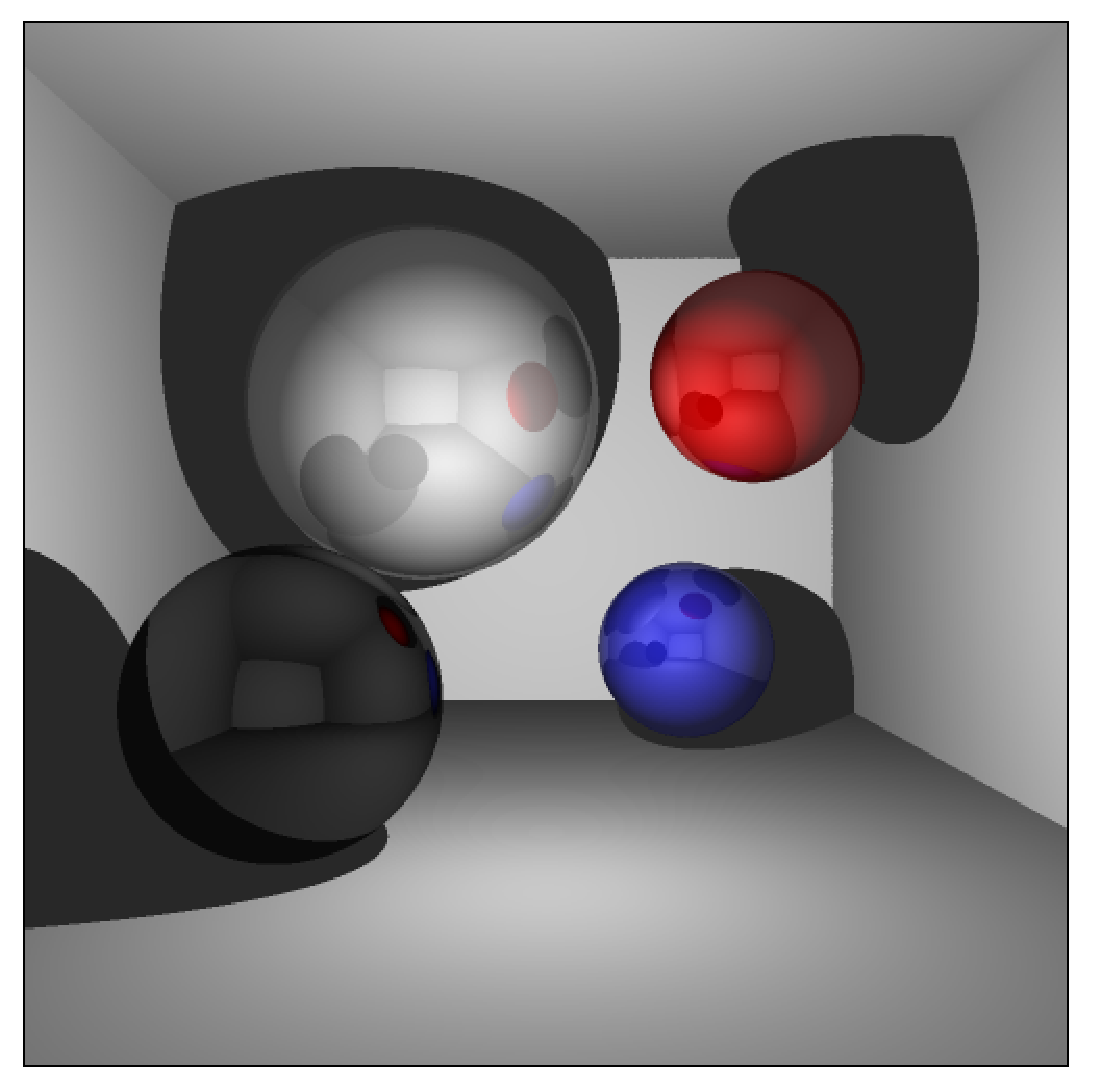
\includegraphics[scale=0.7]{raytracerscreenshot.eps}
\caption{Ray traced 3D scene}
\end{center}
\label{raytracerscreenshot}
\end{figure}

The ray tracer used to test the LJSP compiler includes the following features:
\begin{itemize}
\item An arbitrary number of objects (planes and spheres) can be added to the 3D scene
\item Arbitrarily coloured objects
\item Objects can be made reflective or diffuse
\item Adjustable number of times a light ray gets reflected by reflective objects
\item Both ambient and spot lights
\item Shading \footnote{Varying intensities of light. Visible for example on the floor of the room in the example screen shot in Figure \ref{raytracerscreenshot}.} based on the angle from the surface normal to the light source
\item Antialiasing by downsampling \footnote{This refers to smoothing rugged edges in the scene by first rendering at four times the size of the desired image (width*2 x height*2) before downsizing the result by a factor of four.} 
\end{itemize}

Figure \ref{raytracerscreenshot} shows a rendering of a 3D scene that showcases these features.

% TODO replace underpinning by a better word
\subsection{Mathematical Underpinnings}
The main objects of operation of the ray tracer are rays given by a position and a normalised direction vector: $r = \langle \vec{p}, \vec{d} \rangle$. It is important to note that rays are unlike lines in that they start at position $\vec{p}$ and only extend in the direction given by $\vec{d}$ whereas lines extend to infinity in both directions.

The ray tracer further includes spheres given by a position and a radius: $s = \langle \vec{p}, r \rangle$. It also includes planes given by its normal and the distance from the origin $p = \langle \vec{n}, d \rangle$ and spotlights simply given by a position vector $l = \vec{p}$.

When tracing a ray $r$, the first step is to find the closest object that intersects the path or $r$ if such an object exists. For this, it is necessary to compute both the intersection point and of a ray with both spheres and planes and also obtain the distance to the object, if there is such an intersection point. We will first describe this computations for a ray and a plane before explaining the more complex computation for a ray and a sphere.

% TODO subscripts for all variables
Given the ray $r = \langle \vec{p}, \vec{d_r} \rangle$ and the plane $p = \langle \vec{n}, d_p \rangle$. If the dot product $a$ of the direction vector of the ray and the normal of the plane $\vec{d_r} \cdot \vec{n}$ is equal to $0$, the ray runs parallel to the plane and does not intersect the plane\footnote{Experimental results proved that it is not necessary for successful rendering to consider the case where $r$ lies on the plane.}. If $a \neq 0$ , we treat the ray as a line and calculate $t$, a scalar with the property that $\vec{p} + t*\vec{d_r}$ gives the intersection point of ray and plane. This scalar is given by $-d_p-(\vec{p} \cdot \vec{n}) / (\vec{d_r} \cdot \vec{n})$. If $t < 0$, the plane lies behind the origin of the ray and there is no intersection point of $r$ and $p$.

Calculating the intersection point and $t$ of a ray $r = \langle \vec{p_r}, \vec{d_r} \rangle$ and a sphere $s = \langle \vec{p_s}, r_s \rangle$ is somewhat more complex. The calculation used in the LJSP ray tracer described in the following is mostly based on \cite{physrendering}.

Because the calculations will be made in the object space of $s$, which is the 3D space where the origin lies at $\vec{p_s}$, it is necessary to first translate both $r$ and $s$ to this space. This is very simple in the case of the sphere: Its position is simply set to $(0,0,0)$ as that is how the object space of $s$ is defined. To translate $r$ to the object space of $s$, it is necessary to subtract $\vec{p_s}$ from $\vec{p_r}$. The direction vector of the ray is independent of the position of the ray and does not need to be changed. To make the computation efficient, three temporary variables are now computed that are used repeatedly in the remaining computation:
\begin{equation*}
\begin{aligned}
A &= d_r \cdot d_r\\
B &= 2 \cdot (d_r \cdot p_r)\\
C &= p_r \cdot p_r - r_s \cdot r_s\\
D &= B \cdot B - 4 \cdot A \cdot C
\end{aligned}
\end{equation*}

Calculating the intersection point means solving a quadratic equation that the variable $D$ is the discriminant of. If $D < 0$, the equation has no solution and $r$ and $s$ do not intersect. If $D \geq 0$, two more variables are computed:
\begin{equation*}
\begin{aligned}
t_0 &= \frac{-B-\sqrt{D}}{2 A}\hspace{1.5cm}
t_1 &= \frac{-B+\sqrt{D}}{2 A}
\end{aligned}
\end{equation*}

If both $t_0$ and $t_1$ are less than $0$, there is no intersection point. If one of these two values is less than $0$, the other is returned as $t$. Otherwise the smaller one is returned.

Returning to the process of tracing a ray $r$, after calculating the closest intersection point of the ray with the objects in the scene, the tracing function determines if this intersection point is illuminated by the spot light or if the light is obscured by some other object. It does so by constructing a new ray $r_n = \langle \vec{i}, \vec{d_l} \rangle$ with its position vector $\vec{i}$ being the intersection point and its direction vector $\vec{d_l}$ being a vector going from the intersection point to the light. Again, the closest intersection point of this ray with the objects in the scene is calculated. If there is none, or if it lies behind the light as seen from the ray, the original intersection point is visible from the light, otherwise it is not.

If the point is illumnated by the light, the tracing function next calculates proper shading. If the light from the spot light hights the object that the $r$ intersects with at an angle, the intensity of the light is less than when it hits the object head-on. The intensity of the light hitting the intersection point is calculated by forming the dot product of the objects normal at the intersection point and the direction to the light calculated earlier as $\vec{d_l}$. To imitate ambient light, this value is set to $0.2$, if it is less than that.

If the object hit by the ray $r$ is reflective, the tracing function recurses by tracing the reflection ray before returning a combination of the result of the recursion with the colour of the object. Otherwise it returns the objects colour illuminated with the light calculated in the last section.

% TODO mention test lib and internal forms
\chapter{Implementation}
This chapter will describe the implementation details of the LJSP compiler. It builds on and assumes the previous chapter which describes the parts of the compiler from a theoretical perspective.

We will first give an overview of the files in the repository to enable the reader to find the subsystems described in the design chapter in the code. Following this high-level overview, we will describe the implementation details of a number of compilation stages, filling in the details left out in the last chapter. After @@
% TODO finish this

\section{Structure of the Code}
The code of the LJSP compiler follows a clear structure that separates the code into modules and that makes it easy to find related modules. The necessity for this structure became evident quickly during the development of the compiler, as it was often necessary to edit multiple parts of the code simultaneously.

The code is structured as follows:
\begin{itemize}
\item The entry point of the compiler can be found in \texttt{main.scala}. This files contains functionality to parse and dispatch the arguments the LJSP compiler gets called with by calling the appropriate methods to achieve the desired result.
\item All classes that make up the Abstract Syntax tree can be found in \texttt{AST.scala}. We decided against splitting up this file into a separate file for each language used in the LJSP compiler (LJSP, IR, C, etc.) as that would have lead to unnecessary fragmentation.
\item The compilation stages that make up the LJSP compiler can be found in files with file names starting with a number, e.g. \texttt{03_cps_translation.scala}, optionally followed by a letter that gives a hint as to which stages precede and follow it. These files all contain exactly one object with a name equal to the file name without the number (\texttt{object cps_translation} in the example of CPS-translation) which in turn contain all the methods used in conversion. 
\item The functions that convert ASTs back to specific languages can be found in files that have file names starting with \texttt{code_generation_}. There are five such files in total, one each for every programming language that the LJSP compiler converts to or from: LJSP, IR, asm.js, C and LLVM IR.
\item The file \texttt{run_tests.py} contains the testing framework described further down in the Testing chapter. All other files related to testing can be found in the \texttt{test/} folder.
\item The ray tracer and all files related to it reside in the \texttt{ray_tracer/} folder.
\end{itemize}

%code structure, where to find what in the repo
% code_generation_* as opposite of parser

\section{Implemenation of Various Stages}
% parsing: % uses parser combinator, scala standard lib. maybe write down parser in a mathematical way (the parser combinators
% cps translation: two functions, different types
\section{Structure of the Generated Code}
% closure data structure

\section{Implementation details of the Ray Tracer}
% calls different versions of vectorDotProduct & ray... depending on button clicked
% TODO: describe profiling that shows that raySph... is where the ray tracer spends most of its time. (maybe somewhere else)


\section{Problems encountered \& resolved}
% variables that contain functions, ftables generated at compile time
% memory management in asm.js and C
\section{Experimentation \& Optimisation}
% cps translation different optimisations
% array index vars of type int, others of type double
% (array index vars are all generated, user doesn't see them)

% TODO describe testing
% TODO describe ray tracer
% TODO evaluate choice of scala, maybe not in this chapter (evaluation?)

\chapter{Testing}
% fuzzy testing of compilers
This chapter describes the methods that were used to test the different subsystems of the LJSP compiler. While testing is imperative in all software development, it is especially important in compiler development. The reason for this is that it is usually impossible to determine whether or not a result generated by the compiler is correct simply by looking at the generated code. This is different to other areas of programming like web or user interface development, where a large number of bugs can be found by looking 

During the development of LJSP, two means of testing were being used:
\begin{itemize}
\item A custom testing framework written in Python that covers all of the frontend stages and some of the backend stages.
\item A ray tracer written in JavaScript that was used to test generated asm.js code specifically.
\end{itemize}
The following two sections will describe both systems in detail.

% IR code doesn't get tested because it was a late addition to the compiler and there is only one simple optimisation so far. if development on LJSP continues, an interpreter for IR code will have to be written

\section{Testing using \texttt{run_tests.py}}
% based on the fact described in the design chapter that stages should not affect the result that the program evaluates to
Early on in the development of LJSP, it became necessary to test the output of every front end stage 
\section{Testing using the ray tracer}
% because asm.js evaluates to the same result regardless of
% whether or not it's compiled according to asm.js specification,
% it's possible to add invalid statements and still test the module

% ray tracer to test performance

\chapter{Evaluation}
% ast transformations would be nicer if the compiler generated the subtrees
% from short code snippets instead of creating the objects manually
\section{Evaluation against requirements}
\section{Strengths \& Weaknesses}

\chapter{Conclusions}
\section{Future Work}
\subsection{Implementing a more complete Subset of Scheme}
\subsection{Additional Front Ends}
\subsection{Additional Back Ends}
\subsection{Additional Optimisations}
% IR stages perfect framework for that
\subsection{Better Test Coverage}
% better test coverage
% TODO possibly add: move type inference from C to IR conversion, make IR typed

\chapter{User Guide}
\section{Compiler}
\section{Ray Tracer}
\section{Testing}

\newpage

\chapter{Bibliography}
\begin{thebibliography}{1}
% TODO make links clickable
    \bibitem{githubarchive} {\em GitHub Archive} http://www.githubarchive.org/ accessed on 28.3.2014.
    \bibitem{topgithub} {\em Top Github Languages for 2013 (so far)} http://adambard.com/blog/top-github-languages-for-2013-so-far/ accessed on 28.3.2014
    \bibitem{jsgoodparts} Douglas Crockford (2008) {\em JavaScript: The Good Parts, Unearthing the Excellence in JavaScript}, pp. 101
    \bibitem{sysftal} Morrisett, Greg and Walker, David and Crary, Karl and Glew, Neal (1999). {\em From System F to Typed Assembly Language}, ACM Trans. Program. Lang. Syst.
    \bibitem{brendeich} Foreword by Brendan Eich to {\em Node: Up and Running}. Available at http://chimera.labs.oreilly.com/books/1234000001808/pr02.html accessed on 28.3.2014.
    \bibitem{appel} Andrew Appel (1992). {\em Compiling with Continuations} Cambridge University Press
    % TODO add date and conference name to this reference
    \bibitem{asmjsbenchmark} Alon Zakai, {\em Big Web App? Compile it!} http://kripken.github.com/mloc_emscripten_talk/\#/28 accessed on 30.3.2014
    % TODO google "mozilla is unlocking the power of the web as a platform for gaming" and properly cite
    \bibitem{unreal} TODOTODOTOD
    \bibitem{physrendering} Matt Pharr, Greg Humphreys (2010) {\em Physically Based Rendering, 2nd edition} pp. 116
\end{thebibliography}



\begin{appendices}



\chapter{Programs Listings}

\end{appendices}

\end{document}
